%*****************************************
\chapter{Tables}\label{ch05:tables}
%*****************************************

Excel workbooks are designed to store lots of information and organizing this information so that they display meaningful data can be challenging. Excel has many features that can help organize data and find needed information efficiently. Setting up data as a table from the onset will allows users to sort, filter, total, and subtotal the data easily. In Excel, a table is a collection of data about a particular subject stored in adjacent rows and columns. Tables can improve the look and feel of a workbook. This chapter explores how to best set up Excel tables, how to edit them, and then how to work with them effectively. These skills will be demonstrated in the context of a multi-sheet file that shows national average weather for two very different cities in the United States. Weather data is often voluminous and difficult to summarize since so much is collected every hour of every day and providing meaningful summaries of such data is a useful skill. The skills learned using weather data in this chapter can be be transferred to data found in any discipline or field.

\section{Table Basics}

\begin{center}
	\begin{objbox}{Learning Objectives}
		\begin{itemize}
			\setlength{\itemsep}{0pt}
			\setlength{\parskip}{0pt}
			\setlength{\parsep}{0pt}
			
			\item Understand table structure.
			\item Plan, create, and edit a table.
			\item Freeze rows and columns.
			\item Sort data in a table.
		\end{itemize}
	\end{objbox}
\end{center}

This section reviews the fundamental skills for setting up and maintaining an Excel table. The objective used for this chapter is the construction of a multi-sheet file to keep track of two cities' national weather data for the month of January. Organizing, maintaining, and reporting data are essentials skills for employees in most industries.

Figure \ref{05:fig01} shows the completed workbook that will be demonstrated in this chapter. Notice that this workbook contains three worksheets. The first worksheet lists average weather for January in Portland, Maine. The second sheet lists average weather data for January in a very different climate, Portland, Oregon. The third sheet adds a weekly column to the Portland, Oregon data so that it can be subtotaled by week.

\begin{figure}[H]
	\centering
	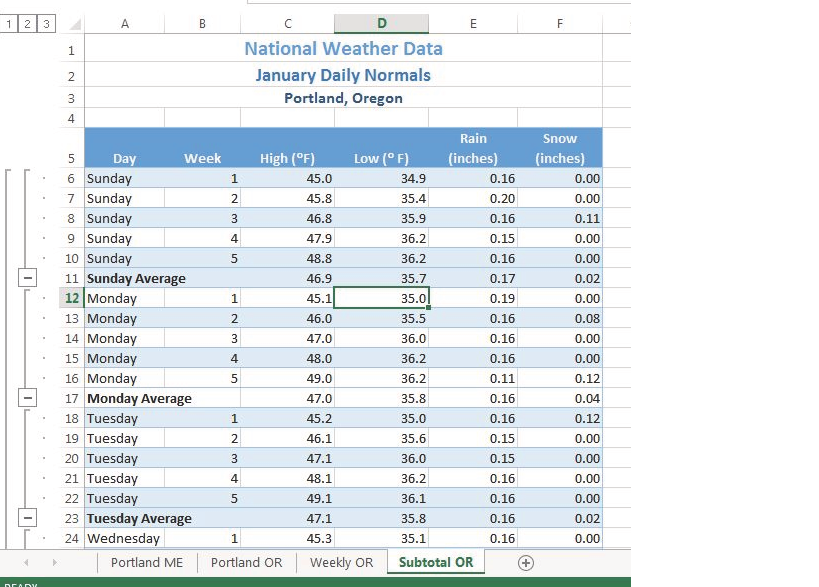
\includegraphics[width=\maxwidth{.95\linewidth}]{gfx/ch05_fig01}
	\caption{Completed National Weather Workbook}
	\label{05:fig01}
\end{figure}

\subsection{Creating a Table}

Data file: \fmtWorkbookName{CH5 Data}

When data is presented in long lists or columns, it helps if the table is set up well. Here are some rules of data-entry etiquette to follow when creating a table from scratch.

\begin{enumerate}
	\item Whenever possible, organize information using adjacent (neighboring) columns and rows.
	\item Start the table in the upper-left corner of the worksheet and work down the sheet.
	\item Do not skip columns and rows just to ``space out'' the information. (To place white space between information in adjacent columns and rows, widen columns, heighten rows, and change the alignment.)
	\item Reserve a single column at the left edge of the table for the table's row headings or identifying information.
	\item Reserve a single row at the top of the table for the table's column headings.
	\item If the table requires a title, put the title in the row(s) above the column headings.
\end{enumerate}

Following these rules will help insure that the sorts, filters, totals, and subtotals applied to the table with return the desired results. With these rules in mind, begin working on the Portland ME worksheet in the National Weather workbook. Notice that the data is in adjacent columns and rows. The upper-left corner of the table is in \textsf{A5} and the titles are above the column headings in Row $ 5 $. Since the set-up of the data looks good, it is time to turn the data range into an Excel table.

\begin{enumerate}
	\item Open data file \fmtWorkbookName{CH5 Data} and save the file as \fmtWorkbookName{CH5 National Weather}.
	\item Click on cell \fmtCellLocation{A5} in the \fmtWorksheetName{Portland ME} sheet.
	\item Click the \fmtButton{Table} button in the \fmtRibbonTab{Insert} tab of the Ribbon.
\end{enumerate}

The diaglog box illustrated in Figure \ref{05:fig02} pops up.

\begin{figure}[H]
	\centering
	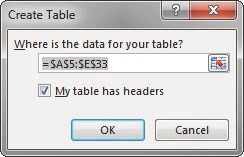
\includegraphics[width=\maxwidth{.95\linewidth}]{gfx/ch05_fig02}
	\caption{Create Table}
	\label{05:fig02}
\end{figure}

\begin{enumerate}
	\item Make sure ``My table has headers'' is checked. Click \fmtButton{OK}.
	\item Click in \fmtCellLocation{arg1}A5 again.
	\item Adjust all column widths so that the complete headings are visible in \fmtCellLocation{Row 5}  with the filter arrows showing. The filter arrows are the down-arrow buttons that will appear in \fmtCellLocation{Row 5} when the table is created. The sorting and filtering procedure is covered later in this chapter.
\end{enumerate}

After this, the worksheet will look like Figure \ref{05:fig03}.

\begin{figure}[H]
	\centering
	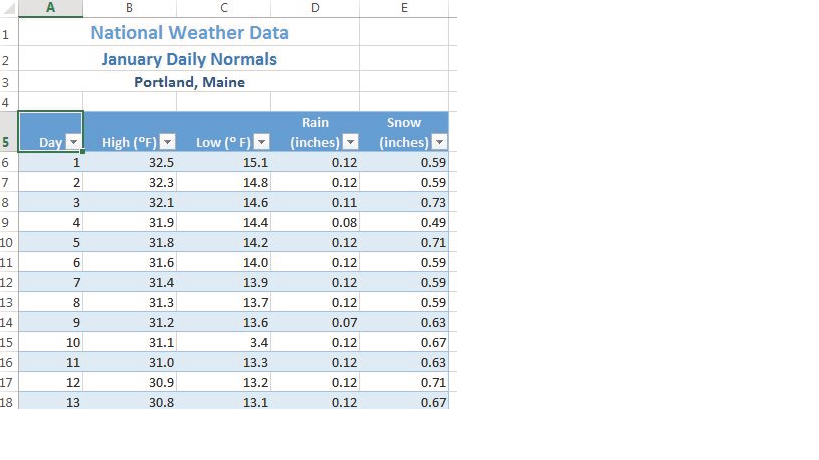
\includegraphics[width=\maxwidth{.95\linewidth}]{gfx/ch05_fig03}
	\caption{Weather Table}
	\label{05:fig03}
\end{figure}

Notice that a new ribbon tab, \fmtRibbonTab{Table Tools Design}, appears when the mouse is clicked inside the table. This ribbon tab contains controls to edit, style, and add functionality to the table. Try these steps again.

\begin{enumerate}
	\item Click on the \fmtWorksheetName{Portland OR} sheet and click in cell \fmtCellLocation{A5}.
	\item Click the \fmtButton{Table} button in the \fmtRibbonTab{Insert} tab of the Ribbon.
	\item Make sure ``My table has headers'' is checked. Click \fmtButton{OK}.
	\item Click in \fmtCellLocation{A5} again.
	\item Adjust all columns widths so that the complete headings in \fmtCellLocation{Row 5} with the filter arrows showing.
\end{enumerate}

\begin{center}
	\begin{sklbox}{Skill Refresher}
		\textbf{Create a Table}
		\\
		\begin{itemize}
			\setlength{\itemsep}{0pt}
			\setlength{\parskip}{0pt}
			\setlength{\parsep}{0pt}

			\item Click on the top left cell in the data.
			\item Click the \fmtButton{Table} button in the \fmtRibbonTab{Insert} tab of the Ribbon.
			\item Make sure ``My table has headers'' is checked. Click \fmtButton{OK}.
			\item Click on the top left cell again.
			\item Adjust all columns widths so the complete headings with the filter arrows are showing.
						
		\end{itemize}
	\end{sklbox}
\end{center}

\subsection{Formatting Tables}

There are many ways to format an Excel table. There are preset colored Table Styles with Light, Medium, and Dark colors. There are also a variety of Table Style Options as listed in Table \ref{05:tab01}.

{\small
	\begin{longtable}{p{1.0in}p{3.00in}} %Max width: 4.25in
		\textbf{Table Style} & \textbf{Description} \endhead
		\hline \\
		Header Row & Top row of the table that includes column headings\\
		Total Row & Row added to the bottom that applies column summary calculations\\
		First Column & Formatting added to the left-most column in the table\\
		Last Column & Formatting added to the right-most column in the table\\
		Banded Rows & Alternating rows of color added to make it easier to see rows of data\\
		Banded Columns & Alternating columns of color added to make it easier to see columns of data\\
		Filter Button & Button that appear at the top of each column that lists options for sorting and filtering\\
		\caption{Table Style Options}
		\label{05:tab01}
	\end{longtable}
}

Add formatting to both of of the Portland weather tables in the following steps.

\begin{enumerate}
	\item Click on the \fmtWorksheetName{Portland ME} sheet.
	\item In the \fmtRibbonTab{Table Tools Design} tab, in the \fmtRibbonGroup{Table Styles} group, click the \fmtButton{More} down-arrow button.
\end{enumerate}

A gallery of table styles will appear as in Figure \ref{05:fig04}.

\begin{figure}[H]
	\centering
	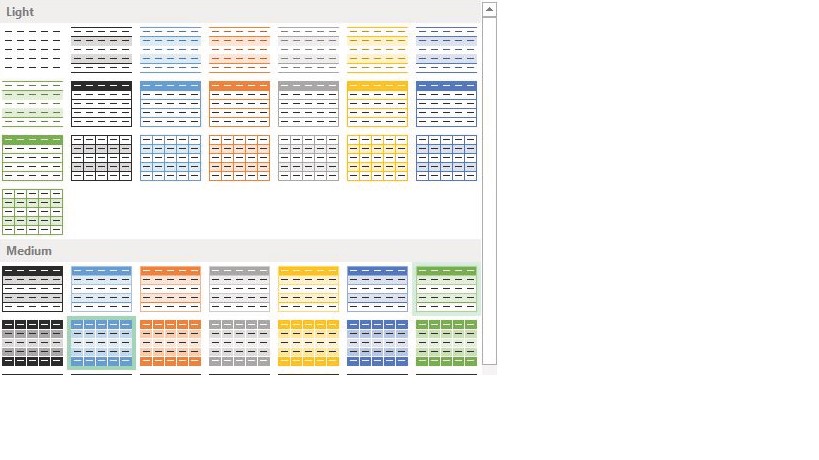
\includegraphics[width=\maxwidth{.95\linewidth}]{gfx/ch05_fig04}
	\caption{Table Styles}
	\label{05:fig04}
\end{figure}

\begin{enumerate}[resume]
	\item In the Table Styles gallery, in the Medium Section, click Table Style Medium $ 7 $.
	\item In the \fmtRibbonGroup{Table Style Options} group in the Ribbon, click \fmtButton{Banded Rows}.
\end{enumerate}

The alternating colored rows will disappear. The data in the table is now more difficult to read.

\begin{enumerate}
	\item Try some of the other options in the Table Style Options group. When finished, check just Header Row, Banded Rows, and Filter Button as in Figure \ref{05:fig05} below.
\end{enumerate}

\begin{figure}[H]
	\centering
	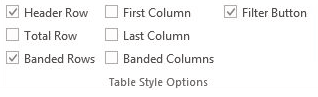
\includegraphics[width=\maxwidth{.95\linewidth}]{gfx/ch05_fig05}
	\caption{Ribbon Table Style Options}
	\label{05:fig05}
\end{figure}

\subsection{Adding Data to Tables}

Over time, new data will need to be added to a table, and that should be added in a blank row. The easiest way to do this is to enter the data in the first blank row below the last row in the table. Then the table can be arranged by sorting. If data must be added in a specific place in the middle of a table, insert a blank row and add the data there.

Add the last three days of the months to the \fmtWorksheetName{Portland ME} and \fmtWorksheetName{Portland OR} worksheets. The following steps walks through this process.

\begin{enumerate}
	\item Click on the \fmtWorksheetName{Portland ME} worksheet.
	\item Click on \fmtCellLocation{A34} (the left-most cell below the last row in the table).
	\item Enter the data from the following table.
\end{enumerate}

\begin{table}[H]
	\centering
	\begin{tabulary}{\linewidth}{CCCCC}
		\hline
		\textbf{Day} & \textbf{High} (\textdegree F) & \textbf{Low} (\textdegree F) & \textbf{Rain} (inches) & \textbf{Snow} (inches) \\
		\hline
		29 & 31.4 & 13.3 & 0.12 & 0.59 \\ 
		30 & 31.6 & 3.4  & 0.08 & 0.47 \\ 
		31 & 31.7 & 13.5 & 0.12 & 0.63 \\ 
		\hline
	\end{tabulary} 
	\caption{Portland, Maine data}
	\label{05:tab02}
\end{table}

Notice that the banded row formatting continues as additional rows are added to the tables.

\begin{enumerate}
	\item Click on the \fmtWorksheetName{Portland OR} worksheet.
	\item Click on \fmtCellLocation{A34} (the left-most cell below the last row in the table).
	\item Enter the data from the following table.
\end{enumerate}

\begin{table}[H]
	\centering
	\begin{tabulary}{\linewidth}{CCCCC}
		\hline
		\textbf{Day} & \textbf{High} (\textdegree F) & \textbf{Low} (\textdegree F) & \textbf{Rain} (inches) & \textbf{Snow} (inches) \\
		\hline
		29 & 48.8 & 36.2 & 0.16 & 0 \\ 
		30 & 49.0 & 36.2 & 0.11 & 0.32 \\ 
		31 & 49.1 & 36.1 & 0.16 & 0 \\ 
		\hline
	\end{tabulary} 
	\caption{Portland, Oregon data}
	\label{05:tab03}
\end{table}

\subsection{Finding and Editing Data}

It is inevitable that data errors which need to be corrected will appear in a table. While it is possible to visually scan through a table to find errors, this can be a tedious and tiresome process. Excel can help with this through the \fmtRibbonButton{Find} command. When using Find, the best practice is to start with the cell pointer in cell \fmtCellLocation{A1} to ensure that all the data in the worksheet is included in the search.

A temperature of $ 3.4 $ degrees was entered erroneously in the \fmtWorksheetName{Portland ME} sheet. It should have been $ 13.4 $. To fix this error, complete the following steps.

\begin{enumerate}
	\item Click on the \fmtWorksheetName{Portland ME} sheet.
	\item Press the \fmtKeystroke{Ctrl}+\fmtKeystroke{Home} keys together to go to the top of the sheet (cell \fmtCellLocation{A1}).
	\item In the \fmtRibbonTab{Home} tab of the ribbon, click on \fmtRibbonButton{Find \& Select} in the \fmtRibbonGroup{Editing Group} and then click \fmtRibbonButton{Find}.
	\item In the \fmtRibbonButton{Find} box, type $ 3.4 $, and then click \fmtButton{Find Next}.
\end{enumerate}

\begin{figure}[H]
	\centering
	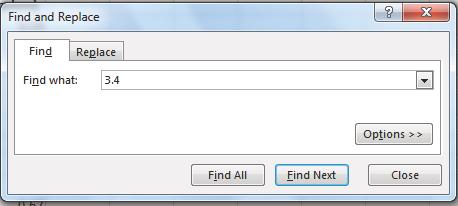
\includegraphics[width=\maxwidth{.95\linewidth}]{gfx/ch05_fig06}
	\caption{Find and Replace}
	\label{05:fig06}
\end{figure}

\begin{enumerate}
	\item Click the \fmtButton{Close} button.
	\item Replace $ 3.4 $ in the Low column for Day $ 10 $ with $ 13.4 $.
	\item Now switch to the \fmtWorksheetName{Portland OR} sheet and find the Snow error of $ .32 $ in Day $ 3 $. Change it to $ 0.12 $. 
\end{enumerate}

\begin{center}
	\begin{sklbox}{Skill Refresher}
		\textbf{Finding and Replacing Data}
		\\
		\begin{itemize}
			\setlength{\itemsep}{0pt}
			\setlength{\parskip}{0pt}
			\setlength{\parsep}{0pt}

			\item In the \fmtRibbonTab{Home} tab of the ribbon, click on \fmtRibbonButton{Find \& Select} in the \fmtRibbonGroup{Editing} Group and then click \fmtButton{Find}.
			\item In the Find box, type the phrase to find then click \fmtButton{Find Next}.
			\item Continue clicking \fmtButton{Find Next} until the phrase is found.
			\item Click \fmtButton{Close} and edit the data.
			
		\end{itemize}
	\end{sklbox}
\end{center}

\subsection{Freeze Rows and Columns}

When panes are ``frozen'' in a worksheet, Microsoft Excel keeps specific rows or columns visible in the table as it is scrolled on the screen. For example, if the first row in the spreadsheet contains labels, that row might be frozen to make sure that the column labels remain visible as the sheet is scrolled down. When scrolling through the weather data, it would be nice to keep column headings visible on the screen. Follow these steps to freeze the headings.

%TODO Start Here
\begin{enumerate}
	\item Click in \textsf{A6}, the left-most cell below the headings row.
	\item Click the View tab in the ribbon.
	\item Select Freeze Panes and then Freeze Top Row (see Figure \ref{05:fig07}).
	\item Scroll up and down the sheet and notice that the headings are always displayed at the top of the table.
\end{enumerate}

\begin{figure}[H]
	\centering
	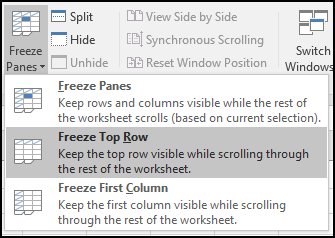
\includegraphics[width=\maxwidth{.95\linewidth}]{gfx/ch05_fig07}
	\caption{Freeze Pane}
	\label{05:fig07}
\end{figure}

To unfreeze the headings:

\begin{enumerate}
	\item Click on the View tab in the ribbon.
	\item Select Unfreeze Panes.
\end{enumerate}

\subsection{Simple Sort}

Content in a table can be sorted alphabetically, numerically, and in many other ways. Sorting helps organize data by one or more columns in the table. Table \ref{05:tab04} describes the different sort orders available for each column of data.

{\small
	\begin{longtable}{p{0.75in}p{1.0in}p{0.65in}p{0.85in}} %Max width: 4.25in
		\textbf{Sort Order} & \textbf{Text} & \textbf{Numbers} & \textbf{Dates} \endhead
		\hline \\
		Ascending & Alphabetical (A-Z) & Smallest to Largest & Chronological (oldest to newest)\\
		Descending & Reverse Alphabetical (Z-A) & Largest to Smallest & Reverse Chronological (newest to oldest)\\
		\caption{Sort Options}
		\label{05:tab04}
	\end{longtable}
}

Suppose it is important to know what the snowiest day was in January in Portland, Maine. One way to find that is to sort the Snow column in Descending order.

\begin{enumerate}
	\item Click on the filter Click arrow to the right of the header Snow (inches) in the Portland ME worksheet.
	\item Click on Click ZA$ \downarrow $ Sort Largest to Smallest. See Figure \ref{05:fig08} below.
\end{enumerate}

\begin{figure}[H]
	\centering
	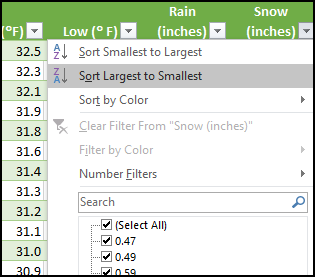
\includegraphics[width=\maxwidth{.95\linewidth}]{gfx/ch05_fig08}
	\caption{Sort by One Column}
	\label{05:fig08}
\end{figure}

If this is done correctly, the snowiest day, January 3rd (in row 6) with 0.73 inches of snow, will be at the top of the list. Notice the filter arrow changes in the snow column to a downward pointing arrow to indicate that the column is sorted in descending order (largest to smallest).

\begin{figure}[H]
	\centering
	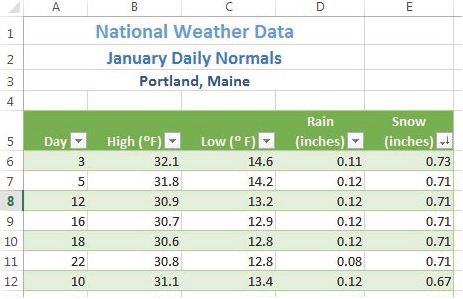
\includegraphics[width=\maxwidth{.95\linewidth}]{gfx/ch05_fig09}
	\caption{Snowiest Days in Maine}
	\label{05:fig09}
\end{figure}

\begin{enumerate}
	\item Now switch to the Portland Oregon sheet and repeat these sort steps to find the snowiest day in Oregon. Check the worksheet with Figure \ref{05:fig10}.
\end{enumerate}

\begin{figure}[H]
	\centering
	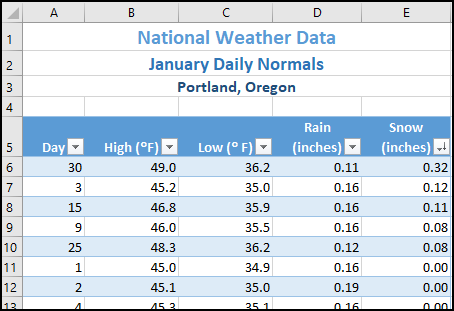
\includegraphics[width=\maxwidth{.95\linewidth}]{gfx/ch05_fig10}
	\caption{Snowiest Days in Oregon}
	\label{05:fig10}
\end{figure}

\begin{center}
	\begin{sklbox}{Skill Refresher}
		\textbf{Sort a Column}
		\\
		\begin{itemize}
			\setlength{\itemsep}{0pt}
			\setlength{\parskip}{0pt}
			\setlength{\parsep}{0pt}

			\item Click on the filter down arrow to the right of the header in the column to be sorted.
			\item Click on the choice AZ$ \downarrow $ or ZA$ \downarrow $ to sort the data in that column.
						
		\end{itemize}
	\end{sklbox}
\end{center}

\subsection{Multi-Level Sort}

Sometimes a table needs to be sorted by more than one column at a time in order to efficiently analyze the data. For example, if the data included several different types of loans from several bank offices, it would need to be sorted by the type of loan and then by bank office name to clearly see the different groups of loans. As another example, if a worksheet included a list of grades for students over their time in high school, the data should be sorted first by student name, then by grade level (freshman, sophomore, junior, and senior) so that each student's grades appear in chronological order.

For the weather data, determine how cold the snow days were in Oregon.

\begin{enumerate}
	\item Click on the Portland OR sheet then click on a cell in the table.
	\item Click on the Data tab in the ribbon and then click the Sort button.
	\item Click the down-arrow for Column and select Snow (inches).
	\item Click the down-arrow for Order and select Largest to Smallest.
	\item To add 2nd level sort, click on the Add Level button in the top left corner of the dialog box.
	\item In the new Then by row, click the down-arrow for Column and select Low (°F).
	\item In the same row, click the down-arrow for Order and select Smallest to Largest. The dialog box should look like Figure \ref{05:fig11}.
\end{enumerate}

\begin{figure}[H]
	\centering
	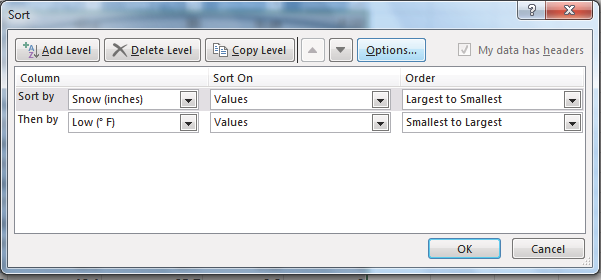
\includegraphics[width=\maxwidth{.95\linewidth}]{gfx/ch05_fig11}
	\caption{Multi-Level Sort}
	\label{05:fig11}
\end{figure}

\begin{enumerate}[resume]
	\item Click OK. The table sort results should look like Figure \ref{05:fig12}. Notice for the two days with $ 0.08 $ inches of snow, the low temp of $ 35.5 $ on Day $ 9 $ is displayed before the low temp of $ 36.2 $ on Day $ 25 $. The lowest of the two was listed first. Also notice that the filter arrows changed on the sorted columns to show how they are sorted.
\end{enumerate}

\begin{figure}[H]
	\centering
	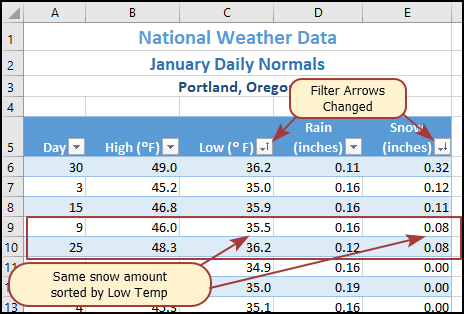
\includegraphics[width=\maxwidth{.95\linewidth}]{gfx/ch05_fig12}
	\caption{Multi-Level Sort Results}
	\label{05:fig12}
\end{figure}

\subsection{Custom Sorts}

In most cases, the data should be sorted in ``typical'' sort order: numbers sorted highest to lowest, words sorted alphabetically, etc. Some data does not make sense when sorted this way. For example, if the days of the week are sorted alphabetically, the result would be : Friday, Monday, Saturday, Sunday, Thursday, Tuesday, and Wednesday. This order would be of no use to anyone! Similarly, the months of the year would not make sense alphabetically.

In the weather data, a column was added for the week in the Weekly OR sheet and changed the days to Sunday through Saturday. This sheet facilitates further analysis of Portland, Oregon's data to see if there are weekly trends in the weather. To look for those trends, sort the Weekly OR sheet by Week and then by Day.

\begin{enumerate}
	\item Click on the Weekly OR worksheet.
\item Click on A5 and insert a table.
\item Click on Sort in the Data tab in the ribbon.
\item Click the down-arrow for Column and select Week.
\item Click the down-arrow for Order and select Smallest to Largest.
\item To add 2nd level sort, click on the Add Level button in the top right corner of the dialog box.
\item In the new Then by row, click the down-arrow for Column and select Day.
\item Click the down-arrow for Order and select Custom List. The dialog box in Figure \ref{05:fig13} will appear on the screen.
\end{enumerate}

\begin{figure}[H]
	\centering
	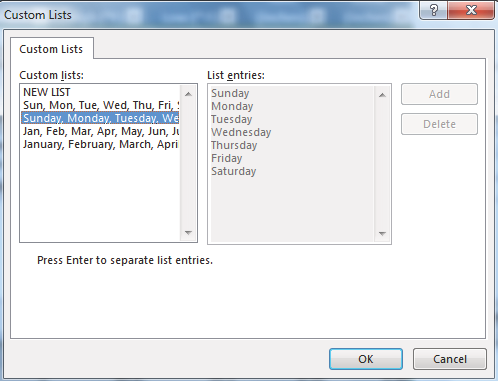
\includegraphics[width=\maxwidth{.95\linewidth}]{gfx/ch05_fig13}
	\caption{Custom Lists}
	\label{05:fig13}
\end{figure}

\begin{enumerate}[resume]
	\item Click on Sunday, Monday, Tuesday, etc. in the Custom lists on the left-side of the dialog box. NOTE: Make sure to select the days of the week spelled out, not the abbreviations for the days of the week.
	\item Click OK. The Sort dialog box should look like Figure \ref{05:fig14}.
\end{enumerate}

\begin{figure}[H]
	\centering
	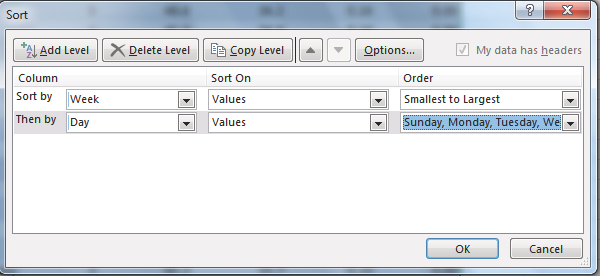
\includegraphics[width=\maxwidth{.95\linewidth}]{gfx/ch05_fig14}
	\caption{Sort Dialog Box}
	\label{05:fig14}
\end{figure}

\begin{enumerate}
	\item Click OK again. The sorted table should now look like Figure \ref{05:fig15}. Notice the data is in Week order and, within each week, in Day order.
\item Save the workbook.
\end{enumerate}

\begin{figure}[H]
	\centering
	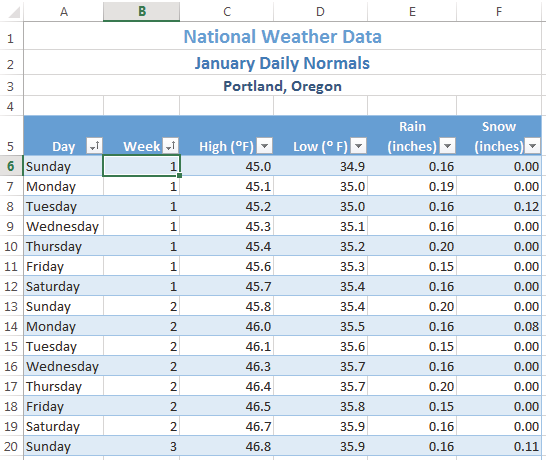
\includegraphics[width=\maxwidth{.95\linewidth}]{gfx/ch05_fig15}
	\caption{Custom Sort}
	\label{05:fig15}
\end{figure}

\begin{center}
	\begin{tkwbox}{Key Take-Aways}
		\textbf{Save}
		\\
		\begin{itemize}
			\setlength{\itemsep}{0pt}
			\setlength{\parskip}{0pt}
			\setlength{\parsep}{0pt}

			\item Tables are made up of adjacent rows and columns of data with a single row of column headings at the top.
			\item Tables are created by clicking in the top left-most cell in the data and selecting Table in the Insert tab of the ribbon.
			\item There are a gallery of styles and options to choose from to format a table.
			\item To add data it is best to add it one row below the bottom of the table. The table can then be resorted to organize the data.
			\item Freezing heading keeps column headings displayed while scrolling through the table data.
			\item Filter arrows in the table headings sort the data by a single column. Use Sort in the Data tab in the ribbon to sort by two or more columns at a time.
			\item Custom Sorts can be used when data needs to be sorted in a special way (\ie Days of the Week).
			
		\end{itemize}
	\end{tkwbox}
\end{center}

\section{Intermediate Table Skills}

\begin{center}
	\begin{objbox}{Learning Objectives}
		\begin{itemize}
			\setlength{\itemsep}{0pt}
			\setlength{\parskip}{0pt}
			\setlength{\parsep}{0pt}

			\item Filter table data.
			\item Add a total row to a table.
			\item Insert subtotals into a table.
			
		\end{itemize}
	\end{objbox}
\end{center}

\subsection{Filtering Data}

When an Excel table is first created, filter arrows appear in all the column headings. Those arrows can be used to sort the data by a single column. These same arrows can also be used to filter or limit the data by narrowing the displayed data within a column. There are many ways to filter data within a column depending on whether the data in the column is text or numeric. Table \ref{05:tab05} contains a few filter examples.

{\fontsize{8}{10} \selectfont
	\begin{longtable}{p{1.5in}p{0.75in}p{1.0in}p{0.75in}} %Max width: 4.25in
		\textbf{Desired Results} & \textbf{Filter Column} & \textbf{Filter} & \textbf{Checkbox} \endhead
		\hline \\
		\multicolumn{4}{l}{\textbf{Text Filters}} \\
		Data for the State of New Jersey (NJ) & State & Equals NJ & NJ \\
		Data for Books that Have Gardening in Their Title & Title & Contains Gardening & \\
		Data for Weather on the Weekend & Day & Equals Saturday or equals Sunday & Saturday and Sunday \\
		\hline \\
		\multicolumn{4}{l}{\textbf{Numeric Filters}} \\
		Data for Income Greater Than $ \$1,000 $ & Income & Greater than $ 1000 $ & \\
		Data for Amount Paid Equal to Zero & Amount Paid & Equals 0.00 & 0.00 \\
		Data for Mortgage and Auto Loans & Loan Type & Equals Mortgage or equals Auto & Mortgage and Auto \\
		\caption{Filter Examples}
		\label{05:tab05}
	\end{longtable}
}

Notice there are sometimes more than one way to filter data (\ie with a filter choice or a checked box). There are also single criteria filters, as well as multi-criteria filters. To start filtering, look at just the first week of data in the Weekly OR sheet.

\begin{enumerate}
	\item Click on the Weekly OR sheet and click on a cell in the table.
	\item Click the filter arrow to the right of the Week heading.
	\item Click the Select All checkbox to deselect all of the checkbox choices.
	\item Click on $ 1 $ to select Week $ 1 $.
	\item Click OK.
\end{enumerate}

The table should look like Figure \ref{05:fig16}. Only $ 7 $ rows of Week $ 1 $ data should be visible in the table. Notice in the Status Bar at the bottom of the screen the message ``7 of 31 records found''. Also notice that the filter arrow in the Week heading has changed to a funnel which indicates that this column is currently filtered.

\begin{figure}[H]
	\centering
	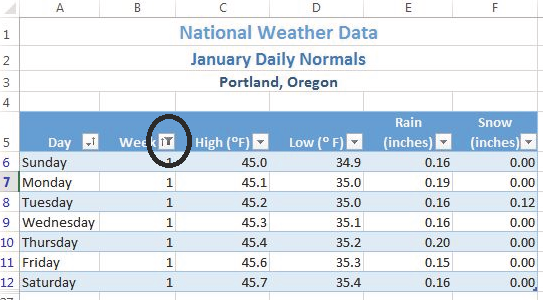
\includegraphics[width=\maxwidth{.95\linewidth}]{gfx/ch05_fig16}
	\caption{Filter}
	\label{05:fig16}
\end{figure}

Follow this procedure to remove the filter.

\begin{enumerate}
	\item Click the funnel next to the Week heading.
	\item Select ``Clear filter from Week''.
\end{enumerate}

\begin{center}
	\begin{sklbox}{Skill Refresher}
		\textbf{Filter a Column}
		\\
		\begin{itemize}
			\setlength{\itemsep}{0pt}
			\setlength{\parskip}{0pt}
			\setlength{\parsep}{0pt}

			\item Click the filter arrow to the right of the heading in the column to be filtered.
			\item Click the Select All checkbox to deselect all of the checkbox choices.
			\item Click on the checkboxes to filter by.
			\item Click OK.
			
		\end{itemize}
		
		\bigskip
		\textbf{Un-Filter a Column}
		
		\begin{itemize}
			\setlength{\itemsep}{0pt}
			\setlength{\parskip}{0pt}
			\setlength{\parsep}{0pt}
			
			\item Click the funnel to the right of the heading in the column to be filtered.
			\item Select Clear filter.
			
		\end{itemize}
	\end{sklbox}
\end{center}

As an example of using a numeric filter, find the days in Portland ME when it was warmer than $ 32 $ degrees in January.

\begin{enumerate}
	\item Click in the Portland ME sheet, then click on a cell in the table.
	\item Click on the filter arrow next to the High heading.
	\item Click on Number filters, then select Greater than. The Custom AutoFilter dialog box will appear on the screen.
	\item Enter $ 32 $ in the space to the right of ``is Greater than''. The Custom AutoFilter dialog box should now match Figure \ref{05:fig17}.
	\item Click OK.
\end{enumerate}

\begin{figure}[H]
	\centering
	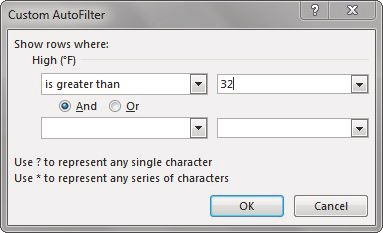
\includegraphics[width=\maxwidth{.95\linewidth}]{gfx/ch05_fig17}
	\caption{AutoFilter Dialog Box}
	\label{05:fig17}
\end{figure}

It is now easy to see that it was only above $ 32 $ degrees for the first three days in January in Maine. Check the table against Figure \ref{05:fig18}.

\begin{figure}[H]
	\centering
	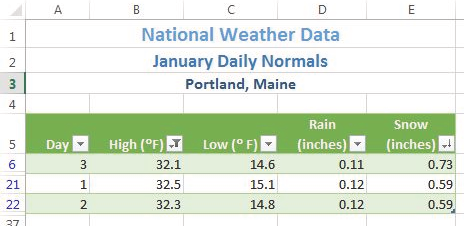
\includegraphics[width=\maxwidth{.95\linewidth}]{gfx/ch05_fig18}
	\caption{Maine Filter Results}
	\label{05:fig18}
\end{figure}

Review sorting and filtering in the following steps.

\begin{enumerate}
	\item Click on the Weekly OR sheet and clear the Day column filter.
	\item Sort the table by Week (smallest to largest).
	\item Filter the table to only show Mondays.
	\item Compare the table results to Figure \ref{05:fig19}.
\end{enumerate}

\begin{figure}[H]
	\centering
	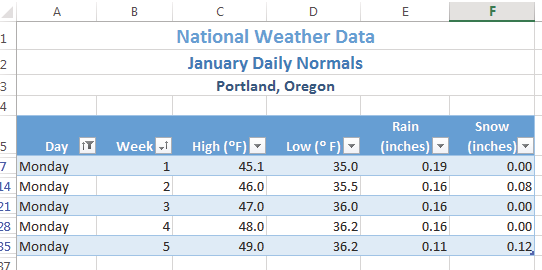
\includegraphics[width=\maxwidth{.95\linewidth}]{gfx/ch05_fig19}
	\caption{Oregon Filter Results}
	\label{05:fig19}
\end{figure}

\subsection{Filtering Using the Slicer}

Beginning in Excel $ 2013 $, slicers were added as another way to filter table data. A slicer is really useful because it clearly indicates what data is shown in the table after the data has been filtered.

Try using the Slicer to filter the Portland OR data table.

\begin{enumerate}
	\item Click on the Portland OR sheet and click in the table.
	\item In the ribbon's Table Tools Design tab, click Insert Slicer.
	\item Click on Day in the Insert Slicers dialog box, and then click OK.
	\item Drag the slicer so that the upper left-hand corner lines up with the top corner of cell G5.
	\item Notice that when a Slicer is inserted, a Slicer Options tab appears on the ribbon. This tab contains links to change the style and size of the entire slicer or the individual slicer buttons.
	\item Click on the Slicer options tab, then click on the More button next to Slicer Styles. The choices in Figure \ref{05:fig20} will show on the screen.
\end{enumerate}

\begin{figure}[H]
	\centering
	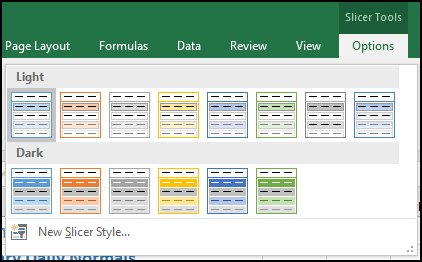
\includegraphics[width=\maxwidth{.95\linewidth}]{gfx/ch05_fig20}
	\caption{Slicer Styles}
	\label{05:fig20}
\end{figure}

\begin{enumerate}
	\item Select the first choice under Dark.
	\item In the Size group on the Slicer Options ribbon (NOT the Buttons group), change the width to $ 1 $ inch.
	\item Click in the table and scroll down to Day $ 15 $ and click the $ 15 $ button to show only the data for January $ 15 $ in the table.
	\item Hold down the \fmtKeystroke{Ctrl} key and click on the Slicer buttons for Days $ 10 $ through $ 14 $. The table should now show the data from Days $ 10-15 $.
	\item Sort the Day column in Ascending order to show the days in order as in Figure \ref{05:fig21}.
\end{enumerate}

\begin{figure}[H]
	\centering
	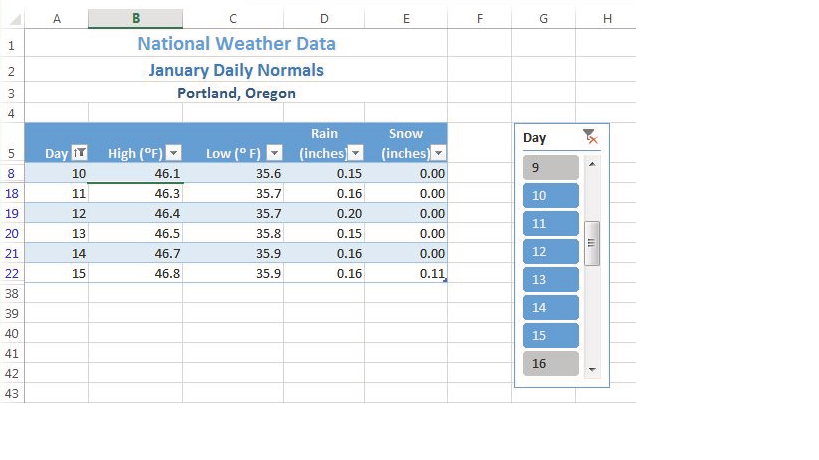
\includegraphics[width=\maxwidth{.95\linewidth}]{gfx/ch05_fig21}
	\caption{Slicer Results}
	\label{05:fig21}
\end{figure}

\subsection{Total Rows}

By adding a total row to the bottom of the table, summary data is easily seen for one or more of the columns. Total rows can be added to tables as a whole or to only those that are filtered. Total rows can easily be toggled on and off as the need for summary data arises.

\begin{enumerate}
	\item Click on the Portland ME sheet and clear the filter from the High column.
	\item Click on the Total Row check box in the Table Style Options group in the Table Tools Design tab in the ribbon.
	\item Scroll to the bottom of the table to the Total Row. Notice the total for the Snow data.
	\item Click on D37 (in the Rain column), and then click the down-arrow that appears to the right of the cell.
	\item Choose Sum to add a sum to the Total Row in the Rain column.
	\item To see the Average rainfall for the month of January, click on the arrow again and choose Average.
	\item Repeat this step in E37 to see the Average snowfall.
	\item Use the Decrease Decimal button in the Home tab of the ribbon to change the decimal places in D37 and E37 to 2. Compare the Total Row to Figure $ 5.22 $.
\end{enumerate}

\begin{figure}[H]
	\centering
	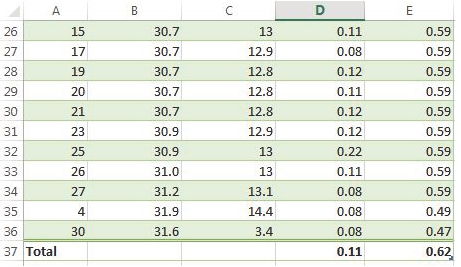
\includegraphics[width=\maxwidth{.95\linewidth}]{gfx/ch05_fig22}
	\caption{Total Row}
	\label{05:fig22}
\end{figure}

Now switch to the Weekly OR sheet and attempt to add a Slicer and Total Row to this table.

\begin{enumerate}
	\item Open the Weekly OR sheet.
	\item Clear the filter from the Day column.
	\item Add a Slicer for the Day column to the sheet.
	\item Move the top left corner of the slicer to H5. Resize it as needed and choose a Slicer Style.
	\item Select Monday through Friday in the Slicer so that Saturday and Sunday data do NOT show in the table.
	\item Add a Total Row that averages the High and Low columns. The averages should be High: $ 47.0 $ and Low: $ 35.8 $. Change the label ``Total'' to ``Average'' by clicking A37 and typing Average.
\end{enumerate}

\begin{center}
	\begin{sklbox}{Skill Refresher}
		\textbf{Add a Total Row}
		\\
		\begin{itemize}
			\setlength{\itemsep}{0pt}
			\setlength{\parskip}{0pt}
			\setlength{\parsep}{0pt}

			\item Click on the Total Row check box in the Table Style Options group in the Table Tools Design tab in the ribbon.
			\item Scroll to the bottom of the table to find the Total Row.
			\item Click in one of the columns in the Total Row, and then click the down-arrow that appears to the right of the cell.
			\item Choose Sum to add a sum to the Total Row in the column.
			\item To see the Average for column, click on the arrow again and choose Average. Some other choices in the Total Row are Count (for words), Count Numbers, Max, and Min.
			
		\end{itemize}
	\end{sklbox}
\end{center}

\begin{center}
	\begin{sklbox}{Skill Refresher}
		\textbf{Add a Slicer}
		\\
		\begin{itemize}
			\setlength{\itemsep}{0pt}
			\setlength{\parskip}{0pt}
			\setlength{\parsep}{0pt}

			\item Click on Insert Slicer in the Table Tools Design tab in the ribbon.
			\item Check the box for the column to which a Slicer is added.
			\item Click OK.
			
		\end{itemize}
	\end{sklbox}
\end{center}

\subsection{Subtotaling}

Subtotals and grand totals can be easily calculated for a column in a table. This is a powerful tool that to quickly display multiple levels of summary data within the table. This can provide Management with a report of higher level summary data one minute, and then can be easily switched back to detailed data the next minute. It is important to save often during this process and follow the steps carefully. It is recommended to make a copy of the data to be subtotaled and place it in a new sheet, so the summary subtotaled data can be separately saved if desired.

In order to subtotal successfully, complete the following steps in order.

\begin{enumerate}
	\item Sort by the column to subtotal on.
	\item Convert the table back to a normal Excel range since a table cannot contain a subtotal.
	\item Subtotal in the Data tab in the ribbon.
	\item To limit the displayed data further, Filter in the Data tab in the ribbon.
\end{enumerate}

The next task is to determine what the weather looks like for each day of the week. Start by to saving data to a new sheet, sort by the days of the week, and then convert the table in order to see the subtotal.

\begin{enumerate}
	\item Click on the Weekly OR sheet.
\item Point at the Weekly OR sheet tab at the bottom of the screen, hold the \fmtKeystroke{Ctrl} key down, and left-drag the sheet to the right until it is past all the existing sheets.
\item When a sheet icon with a + sign is visible, let go of the mouse button and then the \fmtKeystroke{Ctrl} key. A Weekly OR (2) sheet will appear.
\item Right-click on the new Sheet tab, select Rename, type Subtotal OR, and then press \fmtKeystroke{Enter}.
\item Save the file before starting Subtotaling.
\item Remove all filters in the table by clicking the Data tab and then choosing Clear.
\item Now Sort the table by the Day column using a Custom Sort in the Sort button in the ribbon to sort in the order Sunday, Monday, Tuesday, etc. (See Figure \ref{05:fig13} through Figure \ref{05:fig15} for a review of Custom Sorting.)
\item Before adding can subtotals, convert the table back to a regular range. To do this, click Convert to Range in the Table Tools Design tab on the ribbon. (See Figure \ref{05:fig23})
\end{enumerate}

\begin{figure}[H]
	\centering
	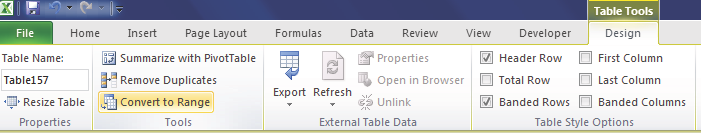
\includegraphics[width=\maxwidth{.95\linewidth}]{gfx/ch05_fig23}
	\caption{Convert to Range}
	\label{05:fig23}
\end{figure}

\begin{enumerate}[resume]
	\item When a box pops up with a warning about converting the table, click Yes.
	\item Because the data is no longer formatted as a table, the slicer will disappear; and the Table Tools Design tab in the ribbon will no longer be available.
	\item Under the Data tab in the ribbon, click Subtotal.
	\item In the Subtotal Window, make the choices shown in the Figure \ref{05:fig24}. It is essential to select the column sorted by in the ``At each change in'' field at the top of the window. Click OK.
\end{enumerate}

\begin{figure}[H]
	\centering
	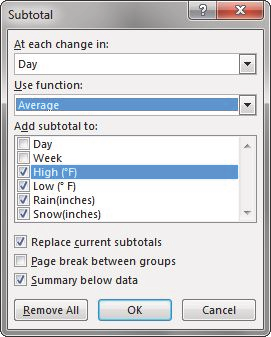
\includegraphics[width=\maxwidth{.95\linewidth}]{gfx/ch05_fig24}
	\caption{Subtotal Window}
	\label{05:fig24}
\end{figure}

The data should look like Figure \ref{05:fig25}. Successful subtotaling shows only one subtotal for each group in the column sorted by. (HINT: If there is more than one Subtotal for the same group (\ie one of the days of the week in the example), then the column was not sorted before subtotaling. Remove the subtotals using the Remove All button in Figure \ref{05:fig24}, sort the table, and then try subtotaling again.)

\begin{figure}[H]
	\centering
	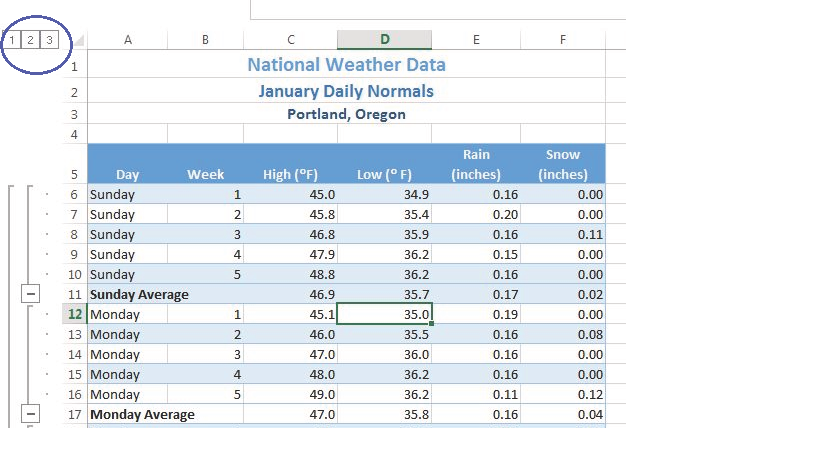
\includegraphics[width=\maxwidth{.95\linewidth}]{gfx/ch05_fig25}
	\caption{Subtotal Results}
	\label{05:fig25}
\end{figure}

Notice the three Outline buttons circled in the upper-left corner of the spreadsheet. These control the amount of subtotaled data that is displayed. Table \ref{05:tab06} describes the different Outline buttons.

{\small
	\begin{longtable}{p{0.50in}p{3.00in}} %Max width: 4.25in
		\textbf{Button} & \textbf{Content Displayed} \endhead
		\hline \\
		Level 1 & Only the grand total\\
		Level 2 & Subtotals and grand total\\
		Level 3 & Individual records, subtotals, and grand total\\
		\caption{Subtotal Outline Buttons}
		\label{05:tab06}
	\end{longtable}
}

Try the three Outline buttons to see the difference in the data displayed.

\begin{enumerate}
	\item Click on the $ 1 $ Outline button in the upper left-hand corner of the sheet.
	\item Only the Grand Average row with averages for High, Low, Rain, and Snow should be visible.
	\item Click on the $ 2 $ Outline button.
	\item The average for each day of the week along with the Grand Average are now visible.
	\item Click on the + Sign button to the left of the Sunday Average row.
	\item This expands just the Sunday Day data and displays the individual records for this subset of the data. Clicking on + Sign buttons will expand a portion of the data at a time. Clicking on – Sign buttons hide a portion of the data at a time.
	\item Click on the $ 3 $ Outline button.
	\item All the individual records along with the subtotals, and Grand Average should be displayed. 
	\item Save the worksheet.
\end{enumerate}

\begin{center}
	\begin{tkwbox}{Key Take-Aways}
		\textbf{Save}
		\\
		\begin{itemize}
			\setlength{\itemsep}{0pt}
			\setlength{\parskip}{0pt}
			\setlength{\parsep}{0pt}

			\item Filtering is an easy way to see a subset of the data. Filtering arrows appear to the right of each column heading when the table has a header row.
			\item Data can be filtered by text or numerically.
			\item A slicer is another way to filter in Excel that provides a set of filtering buttons on the sheet.
			\item Adding a total row to a table is a quick, efficient way to see summary statistics for one or more columns in a table.
			\item Subtotaling provides a way to quickly add totals to groups within a column along with providing a grand total at the bottom of the table.
			\item Subtotal Outline buttons allow users to see add of the subtotaled data, just the totals and grand total, or simply the grand total.
			\item Plus and minus buttons within subtotaling allow a user to expand and hide portions of the subtotaled data.
			
		\end{itemize}
	\end{tkwbox}
\end{center}

\section{Preparing to Print}

\begin{center}
	\begin{objbox}{Learning Objectives}
		\begin{itemize}
			\setlength{\itemsep}{0pt}
			\setlength{\parskip}{0pt}
			\setlength{\parsep}{0pt}

			\item Review options for professional page setup for printing.
			\item Understand how to insert a picture to enhance the visual appearance of a worksheet.
			\item Preview worksheets containing tables to ensure they will print in a professional manner.
			
		\end{itemize}
	\end{objbox}
\end{center}

\subsection{Previewing a Worksheet}

\textit{Data file: CH5 National Weather}

Now that the weather data has been sorted, filtered, and subtotaled as needed, it is time to print the worksheets. Start with the Portland ME worksheet.

\begin{enumerate}
	\item Click on the Portland ME worksheet. 
	\item If needed, use \fmtKeystroke{Ctrl}+\fmtKeystroke{Home} to move to cell A1.
\end{enumerate}

Notice that cells A1, A2, and A3 are not merged and centered over the entire table of data. To fix this, unmerge each of the merged cells, and then merge them again, making sure to include E1, E2, and E3 in the selection.

\begin{enumerate}
	\item Select cell A1 and click the Merge \& Center button. This should split A1 into four cells (A1:D1).
	\item Select the range A1:E1 and click the Merge \& Center button. Cell A1 should now be merged across A1:E1.
	\item Repeat steps 1 and 2 for A2 and A3.
\end{enumerate}

Next preview the worksheet in Print Preview and determine what page setup options need to be set.

\begin{enumerate}
	\item Go to Backstage view and select Print from the menu.
\end{enumerate}

Notice that the table is to the far left of the page with quite a bit of white space on the left. It would look better centered on the page.

\begin{enumerate}
	\item In the Settings section, click the link for Page Setup. This opens the Page Setup dialog box. See Figure \ref{05:fig26}.
\end{enumerate}

\begin{figure}[H]
	\centering
	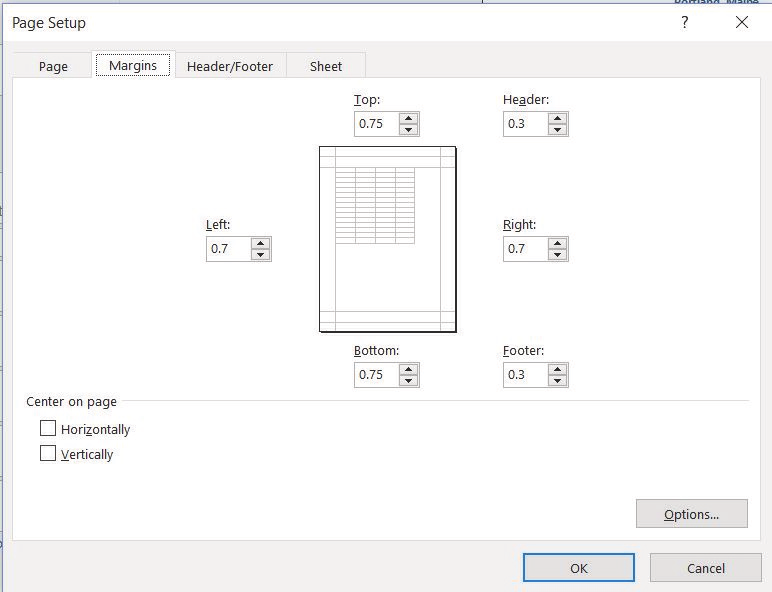
\includegraphics[width=\maxwidth{.95\linewidth}]{gfx/ch05_fig26}
	\caption{Page Setup}
	\label{05:fig26}
\end{figure}

\begin{enumerate}[resume]
	\item Click on the Margins tab.
	\item In the Center on page section, check the box for Horizontally.
	\item Click OK. The table should now be centered horizontally on the page.
	\item Next, add a footer with the workbook filename as well as the worksheet name.
	\item Open the Page Setup dialog box again (see Step 1 above).
	\item Click the Header/Footer tab then click the Custom Footer button.
	\item In the Left section: box type \textit{File:}.
	\item Making sure to leave a space after the colon, click the Insert File Name button.
	\item In the Right section: box type \textit{Worksheet:}.
	\item Making sure to leave a space after the colon, click the Insert Sheet Name button.
	\item The Footer dialog box should look like Figure \ref{05:fig27}. Click the OK button twice to return to Print Preview. Confirm that the footer appears correctly, then exit Backstage View.
\end{enumerate}

\begin{figure}[H]
	\centering
	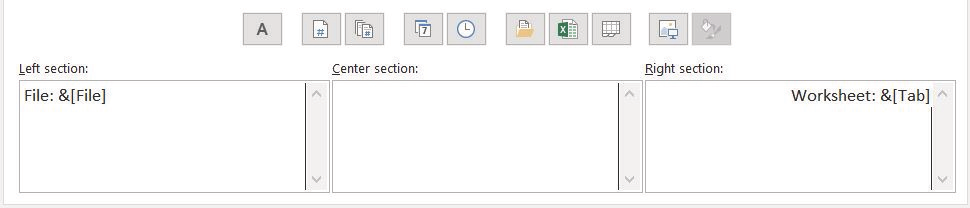
\includegraphics[width=\maxwidth{.95\linewidth}]{gfx/ch05_fig27}
	\caption{Custom Footer}
	\label{05:fig27}
\end{figure}

\subsection{Inserting an Image to Enhance a Worksheet}

Next add a small weather related graphic to the worksheet to enhance its appearance. In Excel, an image file from the local hard drive or downloaded from an online source can be used. In this example, use the graphic available in the data files for this chapter.

\begin{enumerate}
	\item Click the Insert tab on the ribbon.
	\item Click the Pictures button from the Illustrations group. (This inserts an image on the local computer. To search for an online image, click the Online Pictures button.) (See Figure \ref{05:fig28}.)
\end{enumerate}

\begin{figure}[H]
	\centering
	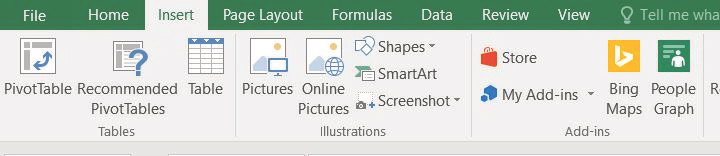
\includegraphics[width=\maxwidth{.95\linewidth}]{gfx/ch05_fig28}
	\caption{Insert Pictures}
	\label{05:fig28}
\end{figure}

\begin{enumerate}[resume]
	\item Navigate to the location where the data files for Chapter $ 5 $ are located and double-click on the Weather image file.
\end{enumerate}

The image now appears on the worksheet, but not in the desired location. It is also slightly larger than desired. (See Figure \ref{05:fig29}.) Move the image to cell E1, then resize it so it does not cover up part of the table.

\begin{figure}[H]
	\centering
	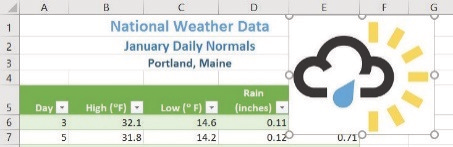
\includegraphics[width=\maxwidth{.95\linewidth}]{gfx/ch05_fig29}
	\caption{Inserted Image}
	\label{05:fig29}
\end{figure}

\begin{enumerate}
	\item Place the pointer in the image so that the the pointer changes to crosshairs. Drag the image so that the top left corner is in cell E1.
	\item Using the resizing handle in the bottom right corner of the image, resize the image so that it does not cover any of the table. Hint: drag diagonally to the left and up.
	\item Check Print Preview again to make sure the worksheet with the image added looks good.
\item Exit Backstage View and save the Excel file.
\end{enumerate}

\subsection{Previewing the Remaining Worksheets}

Before considering this workbook complete finished, confirm that the remaining worksheets are all printing appropriately.

\begin{enumerate}
	\item Click the Portland OR worksheet and go to Print Preview. No changes need to be made to this worksheet. Exit Backstage View.
	\item Click the Weekly OR worksheet and go to Print Preview. Notice that the Slicer is printing on a second page. To fix this, set the Page Scaling to Fit All Columns on One Page.
\end{enumerate}

Notice that the last Slicer button (Saturday) is being cut off. This is because the Slicer height needs to be adjusted.

\begin{enumerate}
	\item Exit Backstage View.
	\item Resize the Slicer so that all of the buttons display.
	\item Return to Print Preview and confirm the worksheet, including the slicer, is printing appropriately. Exit Backstage View.
	\item Click the Subtotal OR worksheet and go to Print Preview.
	\item Using the Page Setup dialog box, center this worksheet horizontally on the page. 
	\item Exit Backstage View.
	\item Save the CH5 National Weather workbook.
	\item Compare the worksheet with the self-check answer key (found in the Course Files) and then submit the CH5 National Weather workbook as directed by the instructor.
\end{enumerate}

\begin{center}
	\begin{tkwbox}{Key Take-Aways}
		\textbf{Save}
		\\
		\begin{itemize}
			\setlength{\itemsep}{0pt}
			\setlength{\parskip}{0pt}
			\setlength{\parsep}{0pt}

			\item When working with Excel workbooks, the final step should always be to review the worksheets in Print Preview to make sure they are printing appropriately.
			\item Images can be added to a worksheet to enhance its appearance. Be sure to resize and move them appropriately so they do not detract from the data.

		\end{itemize}
	\end{tkwbox}
\end{center}

\section{Chapter Practice}

\subsection{Tables for a Tourism Company}

\textit{Data File: PR5 Data}

\begin{figure}[H]
	\centering
	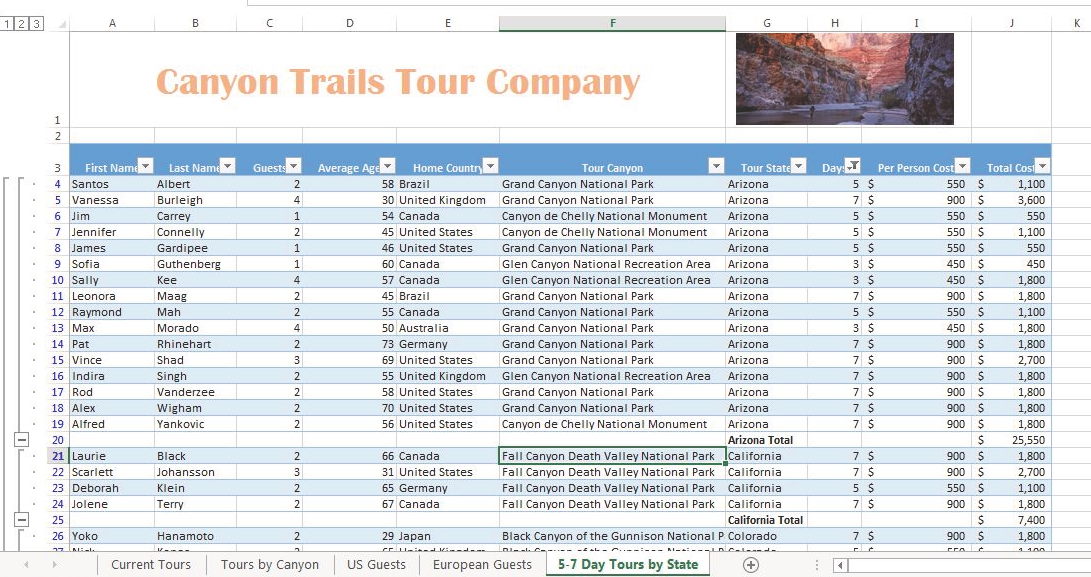
\includegraphics[width=\maxwidth{.95\linewidth}]{gfx/ch05_fig30}
	\caption{Chapter Practice Completed Exercise}
	\label{05:fig30}
\end{figure}

Travel and tour companies need to keep track of client data as well as travel/tour options and tour guides. Keeping up-to-date, accurate records is essential to their bottom line. To run a tour company, employees must be able to manipulate their data quickly and easily. This exercise illustrates how to use the skills presented in this chapter to generate the data needed on a daily basis by a tourism company. See Figure \ref{05:fig30} above.

\begin{enumerate}
	\item Open the data file PR5 Data and save the file as PR5 Canyon Trails.
	\item In Column J, calculate Total Cost (number of \fmtFunction{Guests*Per Person Cost}). Copy the formula down the column.
	\item Format Columns I and J with Currency and no decimal places.
	\item Center all headings in Row 3.
	\item Click in cell A3. Insert a table with headers for the range A3:J53.
	\item Adjust column widths within the table so that all the headings are completely visible.
	\item Rename Sheet $ 1 $ Current Tours. Sort this sheet alphabetically (A to Z) by Last Name.
	\item Make a copy of the Current Tours sheet and rename it Tours by Canyon. Place the Tours by Canyon sheet to the right of the Current Tours sheet. Sort this sheet by Tour Canyon (A to Z), then Home Country (A to Z), and then Last Name (A to Z).
	\item Make another copy of the Current Tours sheet and rename it US Guests. Place the US Guests sheet to the right of the Tours by Canyon sheet. Filter this sheet so that only guests with a Home Country of the United States show. Sort the filtered data alphabetically (A to Z) by Tour State. Add a Total Row that sums the Guests and Total Cost columns.
	\item Make another copy of the Current Tours sheet and rename it European Guests. Place the European Guests sheet to the right of the US Guests sheet. Hide the Average Age column.
	\item Insert a slicer in the European Guests sheet for Home Country. Move the top left corner of the slicer to the top left-hand corner of cell K3. Change the width of the entire slicer to $ 1.65 $ inches.
	\item Select both Germany and the United Kingdom on the slicer. Sort the filtered sheet by Home Country (A to Z) and then Last Name (A to Z).
	\item Make one more copy of the Current Tours sheet and rename it Tours by State. Place the Tours by State sheet to the right of the European Guests sheet. Subtotal the sheet by State, summing the Total Cost column.
	\item Change the name of the Tours by State sheet to $ 5-7 $ Day Tours by State. Filter out $ 3 $ day tours in the table.
	\item On each worksheet, make the following print setup changes.

	\begin{enumerate}
		\item Add a footer with the worksheet name in the center.
		\item Change to Landscape Orientation
		\item Set the scaling to Fit All Columns on One Page
	\end{enumerate}

	\item For any worksheets that print on more than one page, add Print Titles to repeat the first three rows at the top of each page.
	\item Save the PR5 Canyon Trails workbook.
	\item Make sure the sheets are in the following order from left to right: Current Tours, Tours by Canyon, US Guests, European Guests, and $ 5-7 $ Day Tours by State.
	\item Compare the workbook with the self-check answer key (found in the Course Files) and then submit the PR5 Canyon Trails workbook as directed by the instructor.

\end{enumerate}

\section{Scored Assessment}

\subsection{Tables for a Retail Company}

\textit{Data File: SC5 Data}

\begin{figure}[H]
	\centering
	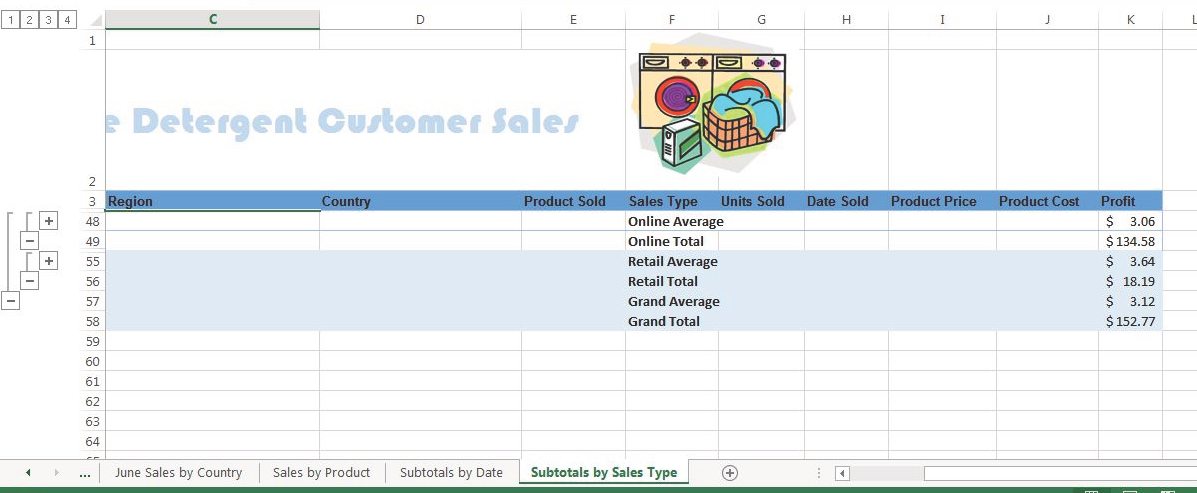
\includegraphics[width=\maxwidth{.95\linewidth}]{gfx/ch05_fig31}
	\caption{Scored Assessment Completed Exercise}
	\label{05:fig31}
\end{figure}

Retail companies with online and in-store sales have a lot of data to keep track of. Keeping track of sales, costs, and profits on a daily basis is essential to making the most of a business. This exercise illustrates how to use the skills presented in this chapter to generate the data needed on a daily basis by a retail company. See Figure \ref{05:fig31} above.

\begin{enumerate}
	\item 1. Open the data file SC5 Data and save the file as SC5 Dynamite Customer Sales.
	\item Click on the Sales sheet. In I4 , enter a \fmtFunction{Vlookup} function that will find the Product Price for the Product in E4 in the table in the Product Table sheet and return it to I4. In the \fmtFunction{Vlookup} function, fill in the required parameters using Figure \ref{05:fig32} below. Copy the \fmtFunction{Vlookup} function down column I.
\end{enumerate}

\begin{figure}[H]
	\centering
	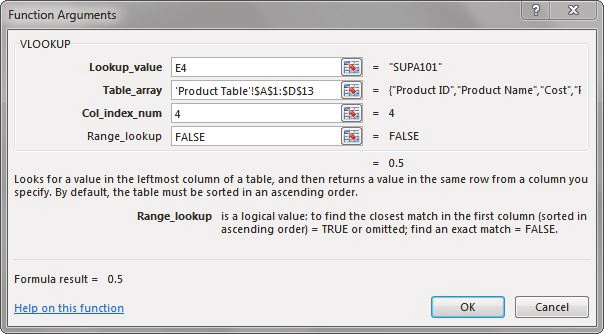
\includegraphics[width=\maxwidth{.95\linewidth}]{gfx/ch05_fig32}
	\caption{\fmtFunction{Vlookup} window}
	\label{05:fig32}
\end{figure}

\begin{enumerate}[resume]
	\item In J4 , enter a \fmtFunction{Vlookup} function that will find the Product Cost for the Product in E4 in the table in the Product Table sheet and return it to J4. This \fmtFunction{Vlookup} function will be the same as the \fmtFunction{Vlookup} function in I4 EXCEPT the COL\_INDEX\_NUM will be $ 3 $ instead of $ 4 $. Copy the function down column J.
	\item In K4, calculate Profit (Product Price – Product Cost). Copy this formula down column K.
	\item Format columns I, J, and K as currency with two decimal places.
	\item Click in cell A3. Insert a table with headers for the range A3:K52. BE CAREFUL HERE: Excel will try to insert a table starting with A2. Be certain the range starts with A3 here.
	\item Make a copy of the Sales sheet and rename it Online Sales by Date. Place this sheet to the right of the Sales sheet. Filter out Retail in Sales Type, so that only Online Sales are displayed. Sort the filtered data by Date Sold (oldest to newest).
	\item Make a copy of the Sales sheet and rename it June Sales by Country. Place this new sheet to the right of the Online Sales by Date sheet. Filter this sheet to only show June dates by using the Date Filter Between. Sort this sheet alphabetically (A to Z) by Country and then alphabetically by Name.
	\item Make another copy of the Sales sheet and rename it Sales by Product. Place this new sheet to the right of the June Sales by Country sheet. Hide the Region column.
	\item Insert a slicer in the Sales by Product sheet for Product Sold. Move the top left corner of the slicer to the top left-hand corner of cell M1. Resize the height of the entire slicer to $ 2.09 $ inches.
	\item Select both DETA100 and DETA200 in the slicer. Sort the filtered sheet by Product Sold. Add a Total Row that includes the overall average for the Product Price, Product Cost, and Profit columns. Change the heading in A53 to Average.
	\item Make a copy of the Sales sheet and rename it Subtotals by Date. Place this new sheet to the right of the Sales by Product sheet. Subtotal the sheet by Date (Oldest to Newest), summing the Profit column. Click the 2 Outline button to show just the subtotals by date and the grand total.
	\item Make one final copy of the Sales sheet and rename it Subtotals by Type. Place this new sheet to the right of the Subtotals by Date sheet. Subtotal the sheet by Sales Type, summing the Profit column.
	\item Add a second subtotal to the Subtotals by Type sheet that subtotals by Type and averages the Profit column. (Hint: uncheck Replace Current Subtotals in the Subtotal dialog box.) Notice that four outline buttons appear with the second subtotal. Figure out which Outline button to click to display both subtotals for Online and Retail and two Grand Totals.
	\item For each worksheet, add a footer with the worksheet name in the center.
	\item Preview each worksheet in Print Preview and make any necessary changes for professional printing. (Hint: Orientation, page scaling, and print titles might need to be used)
	\item Double-check that the sheets are in the following order from left to right: Sales, Online Sales by Date, June Sales by Country, Sales by Product, Subtotals by Date, Subtotals by Sales Type, and Product Table.
	\item Save the SC5 Dynamite Customer Sales workbook.
	\item Submit the SC5 Dynamite Customer Sales workbook as directed by the instructor.
\end{enumerate}
